\documentclass{article}

\usepackage[margin=1in]{geometry}
\usepackage{amsmath}
\usepackage{amssymb}
\usepackage{amsthm}
\usepackage{tikz}
\usepackage{listings}
\usepackage{hyperref}
\usepackage{xcolor}

\usetikzlibrary{arrows.meta, calc, 3d, decorations.pathreplacing}

\definecolor{codebg}{RGB}{248,248,248}
\definecolor{codekw}{RGB}{0,0,180}
\definecolor{codecm}{RGB}{0,128,0}
\definecolor{codestr}{RGB}{163,21,21}

\lstset{
    backgroundcolor=\color{codebg},
    basicstyle=\ttfamily\small,
    keywordstyle=\color{codekw},
    commentstyle=\color{codecm},
    stringstyle=\color{codestr},
    showstringspaces=false,
    breaklines=true,
    frame=single,
    framerule=0.3pt,
    numbers=left,
    numberstyle=\tiny\color{gray},
    xleftmargin=2.5em,
}

\title{Guide 06: Coordinate Frames and Basis Vectors}
\author{web-3d-panel-navigation math curriculum}
\date{}

\newtheorem*{idea}{Key Idea}

\begin{document}
\maketitle

\section{Why this matters}

Almost every geometric computation in this project asks the same question:
\emph{given a panel that is rotated and positioned somewhere in 3D, where do
its axes actually point?} The canonical answer lives in
\texttt{src/zoom-plane-parser.ts:424--429}, where the reference panel's
quaternion is used to recover its right-axis and up-axis in world space, then
those axes are linearly combined with a 2D offset vector to place a hinge
inside the plane's surface. The same maneuver appears in
\texttt{src/camera-controller.ts:59--69} (recover the plane's normal and up so
the camera can sit on the normal axis at the correct distance) and in
\texttt{src/overview-camera.ts:64--72} (same trick, for the overview shot).
Every one of these snippets is doing exactly one thing: \emph{constructing a
local coordinate frame and then describing a point relative to it.} This
guide makes that operation explicit.

\section{Building intuition}

Stand on a tilted ramp and point your right arm. What direction is it pointing
in? Not world-east. Not the global $+x$ axis. It points along whatever
\emph{your} right is, which depends on how the ramp is oriented and which way
you are facing. ``Right'' is meaningful only relative to a frame.

A panel is in the same situation. It is a flat rectangle floating in space,
tilted by some rotation. Three vectors are attached to it:

\begin{itemize}
    \item $\hat{\mathbf{r}}$ -- the panel's own right axis (along its width)
    \item $\hat{\mathbf{u}}$ -- the panel's own up axis (along its height)
    \item $\hat{\mathbf{n}}$ -- the panel's normal (poking out of its surface
          toward the viewer)
\end{itemize}

These three are pairwise perpendicular and each has length one. Together they
form what mathematicians call an \emph{orthonormal frame} attached to the
plane. The center of the plane $\mathbf{c}$ tells us where the frame is; the
three axes tell us how it is oriented.

\begin{center}
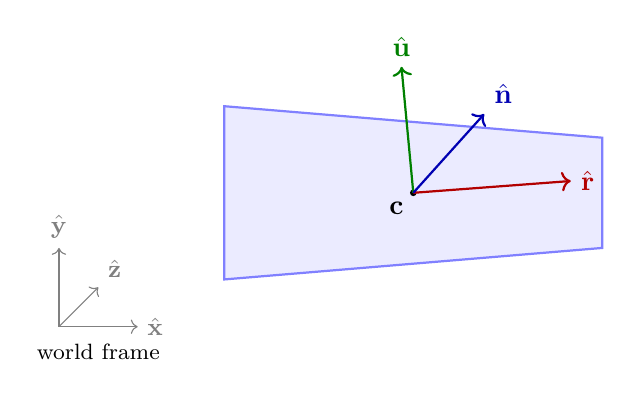
\begin{tikzpicture}[scale=1.0]
  % Tilted plane (parallelogram suggesting a tilted rectangle)
  \coordinate (C) at (0,0);
  \coordinate (A) at (2.4,-0.5);
  \coordinate (B) at (3.0,1.0);
  \coordinate (D) at (-2.4,0.5);
  \coordinate (E) at (-3.0,-1.0);
  % Build a tilted rectangle from C with two in-plane axes
  \coordinate (RT) at (2.4, 0.7);
  \coordinate (LT) at (-2.4, 1.1);
  \coordinate (LB) at (-2.4,-1.1);
  \coordinate (RB) at (2.4,-0.7);
  \fill[blue!8] (LT) -- (RT) -- (RB) -- (LB) -- cycle;
  \draw[blue!50, thick] (LT) -- (RT) -- (RB) -- (LB) -- cycle;
  % Frame at center
  \fill (C) circle (1.2pt);
  \node[below left] at (C) {$\mathbf{c}$};
  % right vector
  \draw[->, thick, red!70!black]   (C) -- ++(2.0, 0.15) node[right] {$\hat{\mathbf{r}}$};
  % up vector
  \draw[->, thick, green!50!black] (C) -- ++(-0.15, 1.6) node[above]  {$\hat{\mathbf{u}}$};
  % normal vector (out of plane, drawn diagonally up-right to suggest 3D)
  \draw[->, thick, blue!70!black]  (C) -- ++(0.9, 1.0)  node[above right] {$\hat{\mathbf{n}}$};
  % World axes off to the side
  \begin{scope}[shift={(-4.5,-1.7)}]
    \draw[->, gray] (0,0) -- (1,0) node[right] {\small $\hat{\mathbf{x}}$};
    \draw[->, gray] (0,0) -- (0,1) node[above] {\small $\hat{\mathbf{y}}$};
    \draw[->, gray] (0,0) -- (0.5,0.5) node[above right] {\small $\hat{\mathbf{z}}$};
    \node[below] at (0.5,-0.1) {\footnotesize world frame};
  \end{scope}
\end{tikzpicture}
\end{center}

The world frame on the lower left is what we always start from: the axes
$\hat{\mathbf{x}}, \hat{\mathbf{y}}, \hat{\mathbf{z}}$ are fixed in space and
have nothing to do with any particular panel. The plane's frame
$\{\hat{\mathbf{r}}, \hat{\mathbf{u}}, \hat{\mathbf{n}}\}$ is just a rotated
copy of the world frame, glued to the plane at the point $\mathbf{c}$.

\begin{idea}
A coordinate frame is two pieces of data: an origin, and three perpendicular
unit vectors. Once you have it, you can address any point either in world
coordinates or in the frame's local coordinates -- and you can convert between
them with a sum of scaled basis vectors.
\end{idea}

\section{The math}

\subsection{Frames, formally}

A \emph{frame} at a point $\mathbf{c} \in \mathbb{R}^3$ is a triple of vectors
$\{\mathbf{e}_1, \mathbf{e}_2, \mathbf{e}_3\}$ that is

\begin{enumerate}
    \item \textbf{orthogonal:} $\mathbf{e}_i \cdot \mathbf{e}_j = 0$ whenever
          $i \neq j$,
    \item \textbf{normalized:} $\|\mathbf{e}_i\| = 1$ for each $i$,
    \item \textbf{spanning:} every vector in $\mathbb{R}^3$ is a unique linear
          combination of $\mathbf{e}_1, \mathbf{e}_2, \mathbf{e}_3$.
\end{enumerate}

Conditions 1 and 2 together say the frame is \emph{orthonormal}. Condition 3
is automatic in $\mathbb{R}^3$ as soon as you have three nonzero pairwise
orthogonal vectors.

The \emph{world frame} (also called the \emph{standard basis}) is the
canonical example:
\[
    \hat{\mathbf{x}} = \begin{pmatrix} 1 \\ 0 \\ 0 \end{pmatrix},
    \qquad
    \hat{\mathbf{y}} = \begin{pmatrix} 0 \\ 1 \\ 0 \end{pmatrix},
    \qquad
    \hat{\mathbf{z}} = \begin{pmatrix} 0 \\ 0 \\ 1 \end{pmatrix}.
\]

\subsection{Rotation matrix columns are images of the standard basis}

This is the single most useful fact in this guide. Let $R$ be a $3 \times 3$
rotation matrix. Multiply $R$ by $\hat{\mathbf{x}}$:
\[
    R \hat{\mathbf{x}}
    \;=\;
    \begin{pmatrix} R_{11} & R_{12} & R_{13} \\ R_{21} & R_{22} & R_{23} \\ R_{31} & R_{32} & R_{33} \end{pmatrix}
    \begin{pmatrix} 1 \\ 0 \\ 0 \end{pmatrix}
    \;=\;
    \begin{pmatrix} R_{11} \\ R_{21} \\ R_{31} \end{pmatrix}.
\]
That is just the first column of $R$. Identically, $R \hat{\mathbf{y}}$ is
the second column and $R \hat{\mathbf{z}}$ is the third. So:

\begin{idea}
The columns of a rotation matrix \emph{are} the basis vectors of the rotated
frame. Applying $R$ to $(1,0,0)$, $(0,1,0)$, $(0,0,1)$ literally peels off
those columns one at a time.
\end{idea}

This is why the project never bothers to construct a $3 \times 3$ matrix when
it wants the rotated axes: it just rotates the standard basis vectors
directly. In code:

\begin{lstlisting}[language=JavaScript]
// Recover the local frame from an Euler rotation
const right = new THREE.Vector3(1, 0, 0).applyEuler(euler);
const up    = new THREE.Vector3(0, 1, 0).applyEuler(euler);
const normal= new THREE.Vector3(0, 0, 1).applyEuler(euler);

// Same idea, but with a quaternion
const right2 = new THREE.Vector3(1, 0, 0).applyQuaternion(q);
const up2    = new THREE.Vector3(0, 1, 0).applyQuaternion(q);
const normal2= new THREE.Vector3(0, 0, 1).applyQuaternion(q);
\end{lstlisting}

Both forms compute the same thing: the columns of the rotation matrix that
$R$ (encoded as Euler angles or as a quaternion) represents.

\begin{center}
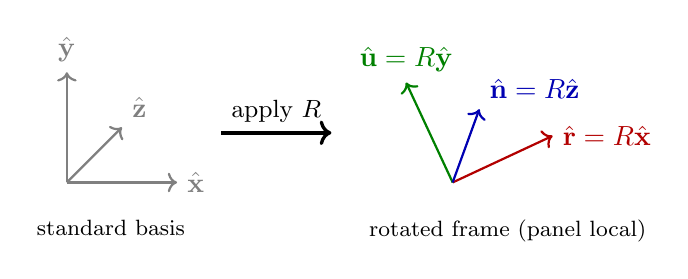
\begin{tikzpicture}[scale=1.4]
  % Standard basis
  \begin{scope}[shift={(-3.0,0)}]
    \draw[->, gray, thick] (0,0) -- (1,0)  node[right]{$\hat{\mathbf{x}}$};
    \draw[->, gray, thick] (0,0) -- (0,1)  node[above]{$\hat{\mathbf{y}}$};
    \draw[->, gray, thick] (0,0) -- (0.5,0.5) node[above right]{$\hat{\mathbf{z}}$};
    \node[below=8pt] at (0.4,-0.05) {\footnotesize standard basis};
  \end{scope}
  % Arrow
  \draw[->, very thick] (-1.6,0.45) -- (-0.6,0.45) node[midway, above] {\small apply $R$};
  % Local frame
  \begin{scope}[shift={(0.5,0)}, rotate=25]
    \draw[->, red!70!black, thick]   (0,0) -- (1,0)  node[right]{$\hat{\mathbf{r}} = R\hat{\mathbf{x}}$};
    \draw[->, green!50!black, thick] (0,0) -- (0,1)  node[above]{$\hat{\mathbf{u}} = R\hat{\mathbf{y}}$};
    \draw[->, blue!70!black, thick]  (0,0) -- (0.5,0.5) node[above right]{$\hat{\mathbf{n}} = R\hat{\mathbf{z}}$};
  \end{scope}
  \node[below=8pt] at (1.0,-0.05) {\footnotesize rotated frame (panel local)};
\end{tikzpicture}
\end{center}

\subsection{Local-to-world for a 2D plane}

A point on the panel has a natural 2D address $(u, v)$, where $u$ is the
horizontal offset from the center and $v$ is the vertical offset. To convert
that to world coordinates, scale each basis vector by the corresponding local
coordinate and add the center:
\[
    \mathbf{w}(u, v) \;=\; \mathbf{c} \;+\; u\,\hat{\mathbf{r}} \;+\; v\,\hat{\mathbf{u}}.
\]
The general 3D form -- if you also let the point sit off the plane along the
normal direction -- is
\[
    \mathbf{w}(u, v, w) \;=\; \mathbf{c} \;+\; u\,\hat{\mathbf{r}} \;+\; v\,\hat{\mathbf{u}} \;+\; w\,\hat{\mathbf{n}}.
\]
Whenever you see code of the shape
\verb|axisA.clone().multiplyScalar(a).add(axisB.clone().multiplyScalar(b))|,
that is this formula. Call it the \emph{basis-weighted sum}: each axis is
scaled by its coefficient and the results are added.

\subsection{The four corners of a panel}

A panel of width $W$ and height $H$, expressed in its own local 2D
coordinates, has four corners:
\[
    \bigl(-\tfrac{W}{2},\; \tfrac{H}{2}\bigr),\;
    \bigl( \tfrac{W}{2},\; \tfrac{H}{2}\bigr),\;
    \bigl( \tfrac{W}{2},-\tfrac{H}{2}\bigr),\;
    \bigl(-\tfrac{W}{2},-\tfrac{H}{2}\bigr).
\]
Promoting these to 3D local points by tacking on a third coordinate of zero
(the panel is flat in its own frame) gives $\bigl(\pm W/2, \pm H/2, 0\bigr)$.
Run each of those through local-to-world and you have the four world-space
corners:
\[
    \mathbf{w}_{\text{corner}} \;=\; \mathbf{c} \;\pm\; \tfrac{W}{2}\,\hat{\mathbf{r}} \;\pm\; \tfrac{H}{2}\,\hat{\mathbf{u}}.
\]
This is exactly the geometry that \texttt{getPlaneWorldCorners} computes,
and we will see the code for it shortly.

\subsection{Orthogonality, briefly}

A rotation matrix $R$ has orthonormal columns by construction, which is
equivalent to saying $R^{\top} R = I$. That means $R^{-1} = R^{\top}$: to
invert a rotation, just transpose it. We will not use that here, but it is
why ``world to local'' is just as cheap as ``local to world.''

\section{In this codebase}

\subsection{Recovering basis vectors from a quaternion}

The headliner pattern, copied verbatim from
\texttt{src/zoom-plane-parser.ts:424--425}:

\begin{lstlisting}[language=JavaScript]
const referenceRight = new THREE.Vector3(1, 0, 0).applyQuaternion(referenceQuaternion);
const referenceUp    = new THREE.Vector3(0, 1, 0).applyQuaternion(referenceQuaternion);
\end{lstlisting}

The panel's orientation is stored as a quaternion. To get the panel's right
axis in world space, we rotate $\hat{\mathbf{x}} = (1,0,0)$ by that
quaternion. To get its up axis, we rotate $\hat{\mathbf{y}} = (0,1,0)$. By
the column-of-$R$ identity, those are the first and second columns of the
underlying rotation matrix -- the rotated frame's right and up.

If we needed the normal we would also rotate $\hat{\mathbf{z}} = (0,0,1)$.
The reference plane in this code path does not need its normal here, because
we are only doing 2D offsets within the plane's surface.

\subsection{The hinge offset is a basis-weighted sum}

Right after recovering those basis vectors, \texttt{zoom-plane-parser.ts:427--429}:

\begin{lstlisting}[language=JavaScript]
const hingeOffset = referenceRight.clone()
  .multiplyScalar(finalOffset[0])
  .add(referenceUp.clone().multiplyScalar(finalOffset[1]));
\end{lstlisting}

This is the local-to-world formula written in JavaScript. The 2D offset
\verb|finalOffset = [u, v]| is converted to a 3D world-space displacement by
\[
    \text{hingeOffset} \;=\; u\,\hat{\mathbf{r}} \;+\; v\,\hat{\mathbf{u}},
\]
where $\hat{\mathbf{r}}$ and $\hat{\mathbf{u}}$ are the reference plane's
own right and up. There is no addition of $\mathbf{c}$ here because this is
a \emph{displacement}, not a position; it is added to the hinge a few lines
later (\texttt{hinge.add(hingeOffset)}).

The unit test file uses this pattern explicitly to anchor the geometry under
test, in \texttt{src/zoom-plane-parser.test.ts:47--56}:

\begin{lstlisting}[language=JavaScript]
function referenceLocalOffset(
  reference: ZoomPlaneConfig,
  x: number,
  y: number
): THREE.Vector3 {
  const quaternion = quaternionFromConfig(reference);
  const right = new THREE.Vector3(1, 0, 0).applyQuaternion(quaternion);
  const up    = new THREE.Vector3(0, 1, 0).applyQuaternion(quaternion);
  return right.multiplyScalar(x).add(up.multiplyScalar(y));
}
\end{lstlisting}

This is the textbook 2D local-to-world: \verb|right * x + up * y|.

\subsection{World corners from local corners}

From \texttt{src/projection.ts:95--119}:

\begin{lstlisting}[language=JavaScript]
const localCorners = [
  new THREE.Vector3(-halfWidth,  halfHeight, 0),  // top-left
  new THREE.Vector3( halfWidth,  halfHeight, 0),  // top-right
  new THREE.Vector3( halfWidth, -halfHeight, 0),  // bottom-right
  new THREE.Vector3(-halfWidth, -halfHeight, 0),  // bottom-left
];

const euler = new THREE.Euler(
  config.rotation[0], config.rotation[1], config.rotation[2]
);
const position = new THREE.Vector3(
  config.position[0], config.position[1], config.position[2]
);

return localCorners.map(corner => {
  const worldCorner = corner.clone();
  worldCorner.applyEuler(euler);
  worldCorner.add(position);
  return worldCorner;
});
\end{lstlisting}

Match this to the formula from the math section. Each local corner is
$(\pm W/2, \pm H/2, 0)$. Applying the Euler rotation is the same as rotating
the local frame onto the world frame: it converts local 3D coordinates into a
\emph{world-space displacement} from the panel center. Adding
\verb|position| is the $+\mathbf{c}$ step. The whole map function is exactly
\[
    \mathbf{w} \;=\; \mathbf{c} \;+\; u\,\hat{\mathbf{r}} \;+\; v\,\hat{\mathbf{u}} \;+\; 0\cdot\hat{\mathbf{n}},
\]
applied four times with $u = \pm W/2$ and $v = \pm H/2$.

\subsection{Camera position along the normal}

From \texttt{src/camera-controller.ts:59--78}:

\begin{lstlisting}[language=JavaScript]
const euler = new THREE.Euler(plane.rotation[0], plane.rotation[1], plane.rotation[2]);

// Plane's normal vector (perpendicular, pointing toward viewer)
const normal = new THREE.Vector3(0, 0, 1);
normal.applyEuler(euler);
normal.normalize();

// Plane's local "up" vector
const planeUp = new THREE.Vector3(0, 1, 0);
planeUp.applyEuler(euler);
planeUp.normalize();

const planeCenter = new THREE.Vector3(
  plane.position[0], plane.position[1], plane.position[2]
);

// Camera position: plane center + (normal * distance)
const cameraPosition = planeCenter.clone().add(normal.clone().multiplyScalar(distance));
\end{lstlisting}

Two of our three frame axes are recovered here: $\hat{\mathbf{n}}$ from
$(0,0,1)$ and $\hat{\mathbf{u}}$ from $(0,1,0)$. The camera position is a
degenerate local-to-world: $u = 0$, $v = 0$, only the normal coordinate is
nonzero,
\[
    \mathbf{p}_{\text{cam}} \;=\; \mathbf{c} \;+\; 0\cdot\hat{\mathbf{r}} \;+\; 0\cdot\hat{\mathbf{u}} \;+\; d\,\hat{\mathbf{n}}.
\]
``Step out from the panel's center, along the panel's own normal, by
distance $d$.''

The same pattern reappears almost identically in
\texttt{src/overview-camera.ts:64--72}: recover the center plane's normal
from its Euler angles, then use that normal as the direction along which the
overview camera will be placed. The local frame of the center plane defines
the overview shot.

\section{Worked examples}

\subsection*{Example 1: a panel rotated 30 degrees about $\hat{\mathbf{y}}$}

Take a panel with
\[
    \mathbf{c} = (0, 0, 0),
    \qquad
    \text{Euler XYZ rotation} = \bigl(0,\; \tfrac{\pi}{6},\; 0\bigr),
    \qquad
    W = 1600,\quad H = 900.
\]
Pure $Y$-rotation by $\theta = \pi/6$ has rotation matrix
\[
    R_Y(\theta) \;=\;
    \begin{pmatrix}
      \cos\theta & 0 & \sin\theta \\
      0          & 1 & 0          \\
      -\sin\theta & 0 & \cos\theta
    \end{pmatrix}
    \;=\;
    \begin{pmatrix}
      \tfrac{\sqrt{3}}{2} & 0 & \tfrac{1}{2} \\
      0                   & 1 & 0            \\
     -\tfrac{1}{2}        & 0 & \tfrac{\sqrt{3}}{2}
    \end{pmatrix}.
\]
The frame's basis vectors are the columns:
\[
    \hat{\mathbf{r}} = \bigl(\tfrac{\sqrt{3}}{2},\; 0,\; -\tfrac{1}{2}\bigr),
    \quad
    \hat{\mathbf{u}} = (0,\; 1,\; 0),
    \quad
    \hat{\mathbf{n}} = \bigl(\tfrac{1}{2},\; 0,\; \tfrac{\sqrt{3}}{2}\bigr).
\]
The top-right corner has local 2D coordinates $(W/2, H/2) = (800, 450)$.
Plugging into the local-to-world formula:
\[
    \mathbf{w}_{TR} \;=\; \mathbf{c} \;+\; 800\,\hat{\mathbf{r}} \;+\; 450\,\hat{\mathbf{u}}
\]
\[
    \;=\; (0,0,0) \;+\; 800\cdot\bigl(\tfrac{\sqrt{3}}{2},0,-\tfrac{1}{2}\bigr) \;+\; 450\cdot(0,1,0)
    \;=\; \bigl(400\sqrt{3},\; 450,\; -400\bigr).
\]
Numerically $400\sqrt{3} \approx 692.82$, so the top-right corner lands at
roughly $(692.82,\; 450,\; -400)$.

\subsection*{Example 2: a hinge offset}

Suppose the reference plane has the same orientation as Example 1 and
\verb|finalOffset = [50, -20]|. Then
\[
    \text{hingeOffset}
    \;=\; 50\,\hat{\mathbf{r}} \;+\; (-20)\,\hat{\mathbf{u}}
    \;=\; 50\bigl(\tfrac{\sqrt{3}}{2}, 0, -\tfrac{1}{2}\bigr) + (-20)(0,1,0)
    \;=\; \bigl(25\sqrt{3},\; -20,\; -25\bigr).
\]
Note that the hinge offset has nonzero components in $x$, $y$, \emph{and} $z$
even though the offset is ``inside the plane.'' That is the whole point of
having a frame: an in-plane offset can have arbitrary world-coordinate
shape, depending on how the plane is oriented.

\subsection*{Example 3: camera placed along the normal}

Same plane as before, with $d = 1200$. The camera position is
\[
    \mathbf{p}_{\text{cam}}
    \;=\; \mathbf{c} \;+\; d\,\hat{\mathbf{n}}
    \;=\; (0,0,0) + 1200\cdot\bigl(\tfrac{1}{2}, 0, \tfrac{\sqrt{3}}{2}\bigr)
    \;=\; \bigl(600,\; 0,\; 600\sqrt{3}\bigr).
\]
Numerically about $(600,\; 0,\; 1039.23)$. The camera is up and to the
right of the world origin even though all we asked for was ``stand back from
the panel along its normal.''

\section{Exercises}

\begin{enumerate}
    \item \textbf{Recover a frame from Euler angles.} A panel has Euler XYZ
          rotation $(0,\; \pi/2,\; 0)$. Compute $\hat{\mathbf{r}},
          \hat{\mathbf{u}}, \hat{\mathbf{n}}$ from the standard basis.

    \item \textbf{Recover a frame from a different rotation.} A panel has
          Euler XYZ rotation $(\pi/2,\; 0,\; 0)$ (rotation about $X$ by
          $90^\circ$). Compute the three frame axes. Which world axis does
          $\hat{\mathbf{u}}$ now coincide with?

    \item \textbf{World corners.} A panel has $\mathbf{c} = (10, 0, -5)$,
          Euler rotation $(0, 0, 0)$, and dimensions $400 \times 200$.
          Compute the four world-space corners.

    \item \textbf{In-plane offset.} Using the panel from Example 1 in the
          worked-examples section, a hover indicator is offset
          \verb|finalOffset = [-100, 60]| from the plane's center. Where is
          its world position?

    \item \textbf{Conceptual: orthonormal columns.} Why must a rotation
          matrix have orthonormal columns? What would go wrong (geometrically)
          if you applied a $3 \times 3$ matrix whose columns were not
          orthonormal to the standard basis vectors?

    \item \textbf{Project-applied: changing local-corner ordering.}
          \texttt{getPlaneWorldCorners} returns its corners in the order
          \texttt{[top-left, top-right, bottom-right, bottom-left]}. Suppose
          a future change reordered them to
          \texttt{[bottom-left, bottom-right, top-right, top-left]}.
          Identify two consequences elsewhere in the project that depend on
          this ordering. (Hint: think about anything that consumes the array
          by index, or anything that interprets ``corner 0'' as a particular
          position.)

    \item \textbf{Project-applied: changing the local-frame convention.}
          The project's ``local right'' is $\hat{\mathbf{x}} = (1,0,0)$ and
          ``local up'' is $\hat{\mathbf{y}} = (0,1,0)$. Suppose you swapped
          conventions: ``local right'' becomes $(0,1,0)$ and ``local up''
          becomes $(1,0,0)$. Trace through what
          \texttt{zoom-plane-parser.ts:424--429} would now compute. Does the
          hinge end up in the same place? If not, why not?
\end{enumerate}

\subsection*{Extension challenges}

\begin{enumerate}
    \setcounter{enumi}{7}
    \item \textbf{Reconstructing the rotation matrix.} You are given only
          $\hat{\mathbf{r}}$, $\hat{\mathbf{u}}$, and $\hat{\mathbf{n}}$ as
          three world-space vectors -- no Euler angles, no quaternion. How
          would you build the $3 \times 3$ rotation matrix that maps the
          standard basis to this frame? Once you have it, how do you go
          backwards (world coordinates to local coordinates)?

    \item \textbf{Cross product as basis completion.} Given just
          $\hat{\mathbf{r}}$ and $\hat{\mathbf{u}}$ (assumed perpendicular
          and unit), explain how to recover $\hat{\mathbf{n}}$ using a
          single operation. Verify this is consistent with the project's
          convention by computing $(1,0,0) \times (0,1,0)$.
\end{enumerate}

\section{Where to next}

In Guide 07 we run this whole picture in reverse: we have world-space points
(like the corners we just computed) and we want to know where they land on
the screen. That is \emph{perspective projection}, world to clip to screen.
Guide 09 then takes the projected corners and fits an axis-aligned screen
rectangle around them -- a bounding box -- which is the basis of the
project's CSS3D-vs-WebGL switching logic. Finally, Guide 11 (the capstone on
hinge tiling) is essentially one extended composition of local frames: the
reference plane has a frame, the relative rotation builds a new frame
hinged off it, the offset rotation perturbs it, and each tiled child plane
gets yet another frame. Every step is local-to-world,
local-to-world, local-to-world, all the way down.

\section*{Appendix: Solutions}

\paragraph{Exercise 1.}
With Euler XYZ $(0, \pi/2, 0)$, $R = R_Y(\pi/2)$:
\[
    R_Y(\tfrac{\pi}{2}) =
    \begin{pmatrix} 0 & 0 & 1 \\ 0 & 1 & 0 \\ -1 & 0 & 0 \end{pmatrix}.
\]
Reading off the columns:
$\hat{\mathbf{r}} = (0, 0, -1)$,
$\hat{\mathbf{u}} = (0, 1, 0)$,
$\hat{\mathbf{n}} = (1, 0, 0)$.
The panel is now facing $+x$; its right is $-z$.

\paragraph{Exercise 2.}
With Euler XYZ $(\pi/2, 0, 0)$, $R = R_X(\pi/2)$:
\[
    R_X(\tfrac{\pi}{2}) =
    \begin{pmatrix} 1 & 0 & 0 \\ 0 & 0 & -1 \\ 0 & 1 & 0 \end{pmatrix}.
\]
$\hat{\mathbf{r}} = (1, 0, 0)$,
$\hat{\mathbf{u}} = (0, 0, 1)$,
$\hat{\mathbf{n}} = (0, -1, 0)$.
The panel's up coincides with the world $+z$ axis.

\paragraph{Exercise 3.}
Zero rotation means the local frame is the world frame:
$\hat{\mathbf{r}} = (1,0,0)$, $\hat{\mathbf{u}} = (0,1,0)$.
With $W/2 = 200$ and $H/2 = 100$:
\begin{align*}
    \text{TL} &= (10,0,-5) + 200(-1,0,0) + 100(0,1,0) = (-190,\; 100,\; -5), \\
    \text{TR} &= (10,0,-5) + 200(1,0,0) + 100(0,1,0)  = (210,\;  100,\; -5), \\
    \text{BR} &= (10,0,-5) + 200(1,0,0) - 100(0,1,0)  = (210,\; -100,\; -5), \\
    \text{BL} &= (10,0,-5) + 200(-1,0,0) - 100(0,1,0) = (-190,\; -100,\; -5).
\end{align*}

\paragraph{Exercise 4.}
With $\hat{\mathbf{r}} = (\tfrac{\sqrt{3}}{2}, 0, -\tfrac{1}{2})$ and
$\hat{\mathbf{u}} = (0, 1, 0)$:
\[
    \mathbf{w} = (0,0,0) + (-100)\,\hat{\mathbf{r}} + 60\,\hat{\mathbf{u}}
              = \bigl(-50\sqrt{3},\; 60,\; 50\bigr).
\]
Numerically about $(-86.60,\; 60,\; 50)$.

\paragraph{Exercise 5.}
Rotation matrices preserve lengths and angles. ``Preserves angles'' means
the rotated $\hat{\mathbf{x}}$ and rotated $\hat{\mathbf{y}}$ remain
perpendicular -- so the rotated columns are pairwise orthogonal.
``Preserves lengths'' means the rotated standard-basis vectors remain unit
length -- so the columns are normalized. Together: orthonormal columns.
If the columns were \emph{not} orthonormal, applying the matrix to the
standard basis would shear the frame: the new ``right'' and ``up'' could be
non-perpendicular, or stretched. A panel transformed by such a matrix would
no longer be a rigid rotated rectangle; it would be sheared and scaled.

\paragraph{Exercise 6.}
Two consequences:
\begin{itemize}
    \item Anything that constructs a polygon from these corners (drawing
          edges, computing perimeter, building a screen-space convex hull)
          would emit edges in the wrong order, potentially producing a
          self-intersecting bowtie shape.
    \item Code that interprets the array by name (``index 0 is the
          top-left, used as the anchor'') silently picks the wrong corner.
          The bounding box (Guide 09) would still be correct, since it
          takes min/max over all four corners regardless of order, but any
          per-corner labeling would break.
\end{itemize}

\paragraph{Exercise 7.}
\texttt{zoom-plane-parser.ts:424--425} would now compute
\verb|new Vector3(0,1,0).applyQuaternion(...)| as ``right'' and
\verb|new Vector3(1,0,0).applyQuaternion(...)| as ``up.'' The roles of
$\hat{\mathbf{r}}$ and $\hat{\mathbf{u}}$ are swapped. The hinge offset
\[
    u\,\hat{\mathbf{r}} + v\,\hat{\mathbf{u}}
\]
would now scale the wrong axis by $u$ and the wrong axis by $v$, so the
hinge ends up in a different world location -- it would be reflected across
the plane's diagonal. This is a useful reminder that ``which axis is right''
is a \emph{convention}, baked in across the whole codebase: \emph{every}
file that recovers a basis vector has to agree.

\paragraph{Exercise 8.}
Place $\hat{\mathbf{r}}, \hat{\mathbf{u}}, \hat{\mathbf{n}}$ as the columns
of a $3 \times 3$ matrix:
\[
    R \;=\; \bigl[\;\hat{\mathbf{r}}\;\bigm|\;\hat{\mathbf{u}}\;\bigm|\;\hat{\mathbf{n}}\;\bigr].
\]
By construction, $R \hat{\mathbf{x}} = \hat{\mathbf{r}}$, and similarly for
$\hat{\mathbf{y}}, \hat{\mathbf{z}}$. To go backwards, use $R^{-1} = R^{\top}$:
the rows of $R$ are the world-frame directions \emph{expressed in local
coordinates}. So a world-space displacement $\mathbf{d} = \mathbf{p} - \mathbf{c}$
has local coordinates
$(u, v, w) = (\hat{\mathbf{r}} \cdot \mathbf{d},\; \hat{\mathbf{u}} \cdot \mathbf{d},\; \hat{\mathbf{n}} \cdot \mathbf{d})$.
Each local coordinate is a dot product of $\mathbf{d}$ with the corresponding
basis vector.

\paragraph{Exercise 9.}
$\hat{\mathbf{n}} = \hat{\mathbf{r}} \times \hat{\mathbf{u}}$. This produces
a unit vector perpendicular to both, with a right-hand-rule orientation.
Sanity check: $(1,0,0) \times (0,1,0) = (0,0,1)$, which is exactly
$\hat{\mathbf{z}}$, matching the project's convention that the third axis
of the local frame is the panel's outward normal.

\end{document}
